\documentclass[addpoints,11pt,a4paper]{exam}
\printanswers
\usepackage{amsmath, amssymb, amsthm}
\renewcommand{\rmdefault}{ppl} % rm
\linespread{1.05}        % Palatino needs more leading
\usepackage[scaled]{helvet} % ss
\usepackage{courier} % tt
\usepackage{eulervm} % a better implementation of the euler package (not in gwTeX)
\normalfont
\usepackage{caption}
\usepackage{csquotes}
\usepackage[T1]{fontenc}
\usepackage{mathrsfs}
\usepackage{comment}
\usepackage{graphicx}
\usepackage{ulem}
\usepackage{paralist}
\usepackage{psfrag}
\usepackage{fullpage}
\usepackage{fancybox}
\usepackage{ifthen}
\usepackage{hyperref}
\hypersetup{
    colorlinks=true,
    linkcolor=blue,
    filecolor=magenta,      
    urlcolor=blue,
}
\usepackage{marvosym}
\usepackage[export]{adjustbox}
\extrawidth{1in}
\usepackage{multicol}
\setlength{\columnsep}{.001cm}
\newcommand{\twopartdef}[4]
{
	\left\{
		\begin{array}{ll}
			#1 & \mbox{if } #2 \\
			#3 & \mbox{if } #4
		\end{array}
	\right.
}
\newcommand{\G}{\mathcal{G}}
\newcommand{\fH}{\mathcal{H}}
\newcommand{\M}{\mathcal{M}}
\title{CS6730 : Assignment 2}
\author{Instructor and TAs}
\date{Release: 27th Mar 2019; {\bf Due: Apr 5th, 11.59pm}}

\begin{document}
\maketitle
\noindent\rule{\textwidth}{1pt}
\begin{itemize}
    \item Submit to {\bf GradeScope a single LaTeX-generated pdf file} containing your solutions. Please type your answers in the solutions blocks in the source LaTeX file of this assignment. 
    \item You are encouraged to collaborate/discuss with other students on this assignment, but write your solutions/code in your own words.
    \item We tried our best to keep coding questions simple so that each coding question should require no more than a page of code (in R say).  
\end{itemize}
\noindent\rule{\textwidth}{1pt}

\begin{questions}
\setcounter{question}{-1}

\question {\sc [mandatory: time to re-search]} The research paper assignment will be done collaboratively in teams of 4 students each - its deadline will be later in the course, and its evaluation will be based on a critique written by each member in his/her own words (70\%) and a team presentation (30\%). For now, please provide your 
\begin{parts}
\part team members and team name, and 
%\begin{solution}
%\end{solution}
\part the single research paper your team has chosen. 
%\begin{solution}
%\end{solution}
\end{parts}
Some example papers are in the course moodle, but feel free to choose any other research paper with some component of probabilistic graphical modeling.

\question[5] {\sc [Junction Tree gets a tune-up]} Let $H=({\mathcal X}, E)$ be a chordal Markov network, and let $T=(C,F)$ be a junction tree for $H$. Let $\beta_c$ for $c \in C$ be a set of (locally) calibrated potentials, i.e. for all $(i,j) \in F$, we have that 
\[\sum_{C_i \setminus S_{i,j}} \beta_i(C_i) = \sum_{C_j \setminus S_{i,j}} \beta_j(C_j),\]
where $S_{i,j}=C_i\cap C_j$. Show that for all $i,k \in C$ (not necessarily neighbors in $T$), we have that if $a\in C_i$ and $a\in C_k$, 
\[ \sum_{C_i\setminus\{a\}} \beta_i(C_i) = \sum_{C_k\setminus\{a\}} \beta_k(C_k)\]
%\begin{solution}
%\end{solution}
(Note: After a junction tree algorithm is run, we can compute $P(X_i)$ by choosing {\bf any} clique $c$ containing $X_i$ and marginalizing out all other variables from $\beta_c$ -- this works as the $\beta_c$ of different cliques $c$ are each valid (unnormalized) marginals of the same (original) joint distribution. This question shows that this behavior also holds true for any set of general factors/potentials $\beta_c$ as long as they are calibrated (including {\it pseudo-marginal} potentials $\beta_c$ that are not marginals for any valid joint distribution over $\mathcal{X}$, and which have applications in variational inference).)

\question[10]{\sc [Toying around with MCMC::MH]} Use normal distribution centered at the current state of the chain as a proposal distribution in the Metropolis-Hastings algorithm to sample from the $Gamma(\theta,1)$ distribution when $\theta$ is a non-integer that is at least $2$. 
\begin{parts}
\part[3] Write down the acceptance probability (after all simplifications). What properties do you need to verify to confirm your method reaches the right stationary distribution after running for a sufficiently long time? Show your verification.
%\begin{solution}
%\end{solution}
\part[4] Provide your code that simulates 1000 values from ${\sf Gamma}(5.5, 1)$, and show the trace plots, and the histogram of $X_n$ (with the gamma density overlaid).
%\begin{solution}
  %\begin{lstlisting}
  %Put your code here.
  %\end{lstlisting}
%\end{solution}
\part[3] How did you choose your burn-in time? Report it along with your acceptance rate during the burn-in vs. sample collection periods. How did these values change as a function of the variance parameter of your normal distribution, and what do you think is the optimal variance for fast convergence?
%\begin{solution}
%\end{solution}
\end{parts}

\question[10]{\sc [Hard-core with MCMC::Gibbs]} \\ 
\begin{minipage}{0.35\textwidth}
 \begin{center}
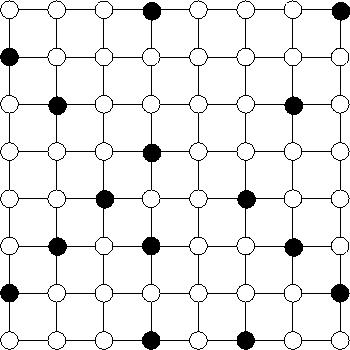
\includegraphics[scale=0.3]{hardcore.jpg}     
 \end{center}
 \end{minipage}
 \begin{minipage}{0.6\textwidth}
Consider a (non-complete) connected graph \textit{G = (V, E)} such as the one shown with $n=|V|$. Now each vertex in $V$ gets either mapped to $0$ or $1$, where we only consider the following set $C \subset \{0,1\}^n$ of admissible configurations characterized by the property that pairs of adjacent vertices {\bf cannot both} take the value $1$ (see figure where black denotes 1).

Now, we want to pick one of the admissible configurations ${\mathbf x} \in C$ ''at random''. That is, we consider the (discrete) uniform distribution $\pi$ on $C$, i.e. $\pi_{\mathbf{x}}=\frac{1}{|C|} ~~\forall~{\mathbf{x}} \in C$. 
 \end{minipage}
 \begin{parts}
 \part[3] Write down the edge potentials of the undirected graphical model for this problem, and a Gibbs sampling algorithm for sampling from this model (including how you derived the associated conditional $P(X_i | X_{-i})$). Does your algorithm need to know the partition function $|C|$?
%\begin{solution}
%\end{solution}
\part[3] Is the Markov chain you set up irreducible and aperiodic? Does your chain admit a distribution that satisfies detailed balance? If it simplifies your proof, assume here that your Gibbs sampling routine employs ``random scan'' (pick a random $i$ from $1,\ldots,n$ and then make a move based on $P(X_i | X_{-i})$ in each epoch) instead of ``systematic scan'' (cycle through all $i$ from $1$ to $n$ in each epoch). 
%\begin{solution}
%\end{solution} 
\part[4] Provide your code and trace plots (of some functions that each map a configuration to a real value that helps visualize how well the chain is mixing). Plot the burn-in time you chose as a function of the size of the grid graphs you used. We didn't ask about the empirical acceptance rate here as it is always 100\% for Gibbs sampling - prove that it is so under the same ``random scan'' epoch assumption above.
%\begin{solution}
  %\begin{lstlisting}
  %Put your code here.
  %\end{lstlisting}
%\end{solution}
\end{parts}

\question[10]{\sc [Block now, collapse later]}
Under some conditions, it is useful to partition the random variables into \enquote{blocks}, and consider these blocks as ``super'' random variables to do Gibbs sampling on. The same logic for Gibbs sampling applies here as well to show that this also has the stationary distribution equal to $P$. Sometimes implementing a block Gibbs sampling step takes strictly more computation than standard Gibbs sampling, but it helps by aiding a faster convergence to the stationary distribution.
\begin{parts}
\part[3] For Model (a) given below, what is the computational complexity (give an upper bound) of one complete cycle of Gibbs sampling, and of one complete cycle of block Gibbs sampling with $\frac{n}{k}$ blocks of $k$ variables each? Assume ``systematic scan'' Gibbs sampling (see previous question) is done in each epoch.

{\bf Model (a)}: Let $\Phi$ be a set of factors over $X=(X_1,\ldots,X_n)$. Let \\
$P(X) = \frac{1}{Z} \prod_{\phi \in\Phi} \phi(D_\phi)$,\\
where $D_\phi$ is the scope of factor $\phi$. Let each random variable $X_i$ take values in $\{0,1,\ldots, c-1\}$. Let each variable $X_i$ occur in at most $b$ factors. Let cardinality of $D_\phi$ be upper bounded by $a$ for any factor $\phi \in \Phi$. 
%\begin{solution}
%\end{solution}

\part[7] Try both Gibbs and block Gibbs sampling approaches for Model (b) given below (group the strongly coupled random variables $X_1,X_2$ into a block and $X_3,X_4$ into another block). Provide code, and show how long your code took to reach stationary distribution with or without blocking? Provide intuition on why sampling from Model (b) with or without blocking resulted in different convergence rates. 

{\bf Model (b):} Consider four random variables with distribution\\
$P(X_1,X_2,X_3,X_4)=\frac{1}{Z}\psi(X_1,X_2)\psi(X_3,X_4)\phi(X_2,X_3)$, \\
where 
$\psi=\begin{bmatrix} 
100 & 1 \\
1 & 100 
\end{bmatrix}$ and 
$\phi=\begin{bmatrix} 
2 & 1 \\
1 & 2 
\end{bmatrix}$.

(Note: Block Gibbs sampling is different from collapsed Gibbs sampling, where certain variables are integrated out. We may see collapsed Gibbs sampling in a later assignment/tutorial.)
%\begin{solution}
  %\begin{lstlisting}
  %Put your code here.
  %\end{lstlisting}
%\end{solution}
\end{parts}

\end{questions}
\end{document}
